\chapter{Analyse mit CryptoMiniSat}
\label{chp:analyse}

Die im letzten Kapitel erstellte konjunktive Normalform wird in diesem Kapitel für eine Analyse verwendet.

4.2.0\\
4.4.0\\
4.5.3\\

generell urbildberechnung \ref{sec:urbildberechnung}\\
unterschied zur Inittialwertberechnung \ref{sec:initialwertberechnung}

mehrere durchläufe mit cryptominisat\\
ein durchlauf besteht aus mehreren lösungsversuchen mit jeweils einem bit vorgabe mehr\\
~\\
reale werte nur per assumptions, um allgemeine klauseln zu erhalten\\
reale werte sind initialwerte (konstanten), hash und 12 byte vom padding\\
52 Byte lang: Das ist eine Eingabe aus der ein Hash erstellt wird.\\
Durch Padding werden 12 Byte angehangen: per assumption vorgeben.
hash ist: 27931f0e 7e53670d dbec1a1c e23e21b4 663c63c0 d17117ee 1a934bc0 c294dbe9\\
interaktive Ruby-Konsole: IRB.\\
\\
\begin{figure}[!h]
  \centering
  \begin{lstlisting}[]
  require 'digest'
  Digest::SHA256.hexdigest 'Das ist eine Eingabe aus der ein Hash erstellt wird.'
   => "27931f0e7e53670ddbec1a1ce23e21b4663c63c0d17117ee1a934bc0c294dbe9"
  \end{lstlisting}
  \caption{Ruby - \glos{sha256}}
  \label{fig:ruby-sha256}
\end{figure}
~\\
bei jeder lösung werden klauseln rausgeschrieben\\
kein unterschied zwischen redundant und irredundant - beides wird analysiert\\
im folgenden die schritte der analyse:

\section{Aussortieren bekannter und doppelter Klauseln}
\label{sec:ana:rem_double}

Da die Entscheidung, ob eine XOR-Unterstützung vorliegt, beim Kompilieren getroffen werden muss, werden die bekannten Klauseln
mit dem Programm "`dimacsprinter"' nach jedem Lösungsversuch und der darauf folgenden Analyse in zwei Dateien im DIMACS-Format
ausgegeben. Die eine Datei enthält dabei die Klauselmenge ohne XOR-Unterstützung während die andere Datei die Klauselmenge für
eine XOR-Unterstützung enthält. Das Programm "`clausecollector"' liest beide Dateien beim Start ein und führt die Klauselmengen
zusammen. Da CryptoMiniSat XOR-Klauseln akzeptiert, diese jedoch intern in normale Klauseln umrechnet, enthalten auch die
extrahierten Klauseln keine XOR-Klauseln. Der Parser für das DIMACS-Format konvertiert deshalb ebenfalls XOR-Klauseln in normale
Klauseln.

Abgelegt werden die bekannten Klauseln in einem "`set"'. Diese Datenstruktur ermöglicht die Suche nach einer Klausel in logarithmischer
Zeit im Bezug zur Anzahl der darin enthaltenen Klauseln. So kann effizient geprüft werden, ob eine extrahierte Klausel schon bekannt ist.
Neue Klauseln aus der irredundanten und der redundanten Klauselmenge werden ebenfalls jeweils in einem "`set"' gesammelt wodurch die
Klauselmenge automatisch sortiert wird und doppelte Klauseln wegfallen. Abschließend werden die neuen Klauseln aus der irredundanten und
der redundanten Klauselmenge jeweils in in eine DIMACS-Datei zur weiteren Analyse geschrieben.
\section{Erkennen und normalisieren modulspezifischer Klauseln}
\label{sec:ana:module}

Nach dem Aussortieren der schon bekannten Klauseln werden die neuen Klauseln den einzelnen Modulen zugeordnet. Durch die hierarchische Anordnung
muss beachtet werden, dass eine Klausel mehreren Modulen zugeordnet werden kann. Sinnvoll ist es jedoch, die Klausel nur dem Modul zuzuordnen,
das in der Hierarchie möglichst weit unten steht. Wird eine Klausel für einen Addierer gefunden, kann diese Klausel so zukünftig für alle Addierer
genutzt werden, während sie im Modul für die vollständige Kompressionsfunktion nur für den einen speziellen Addierer gelten würde. Um diese
Zuordnung zu realisieren, erhält jedes Modul ein Level. Im hierarchischen Aufbau muss das Level eines Moduls dabei höher sein als das höchste Level
der verwendeten Module. Die vergebenen Level sind in Abbildung \ref{fig:sha256_module_level} dargestellt.
\begin{figure}[!h]
  \centering
  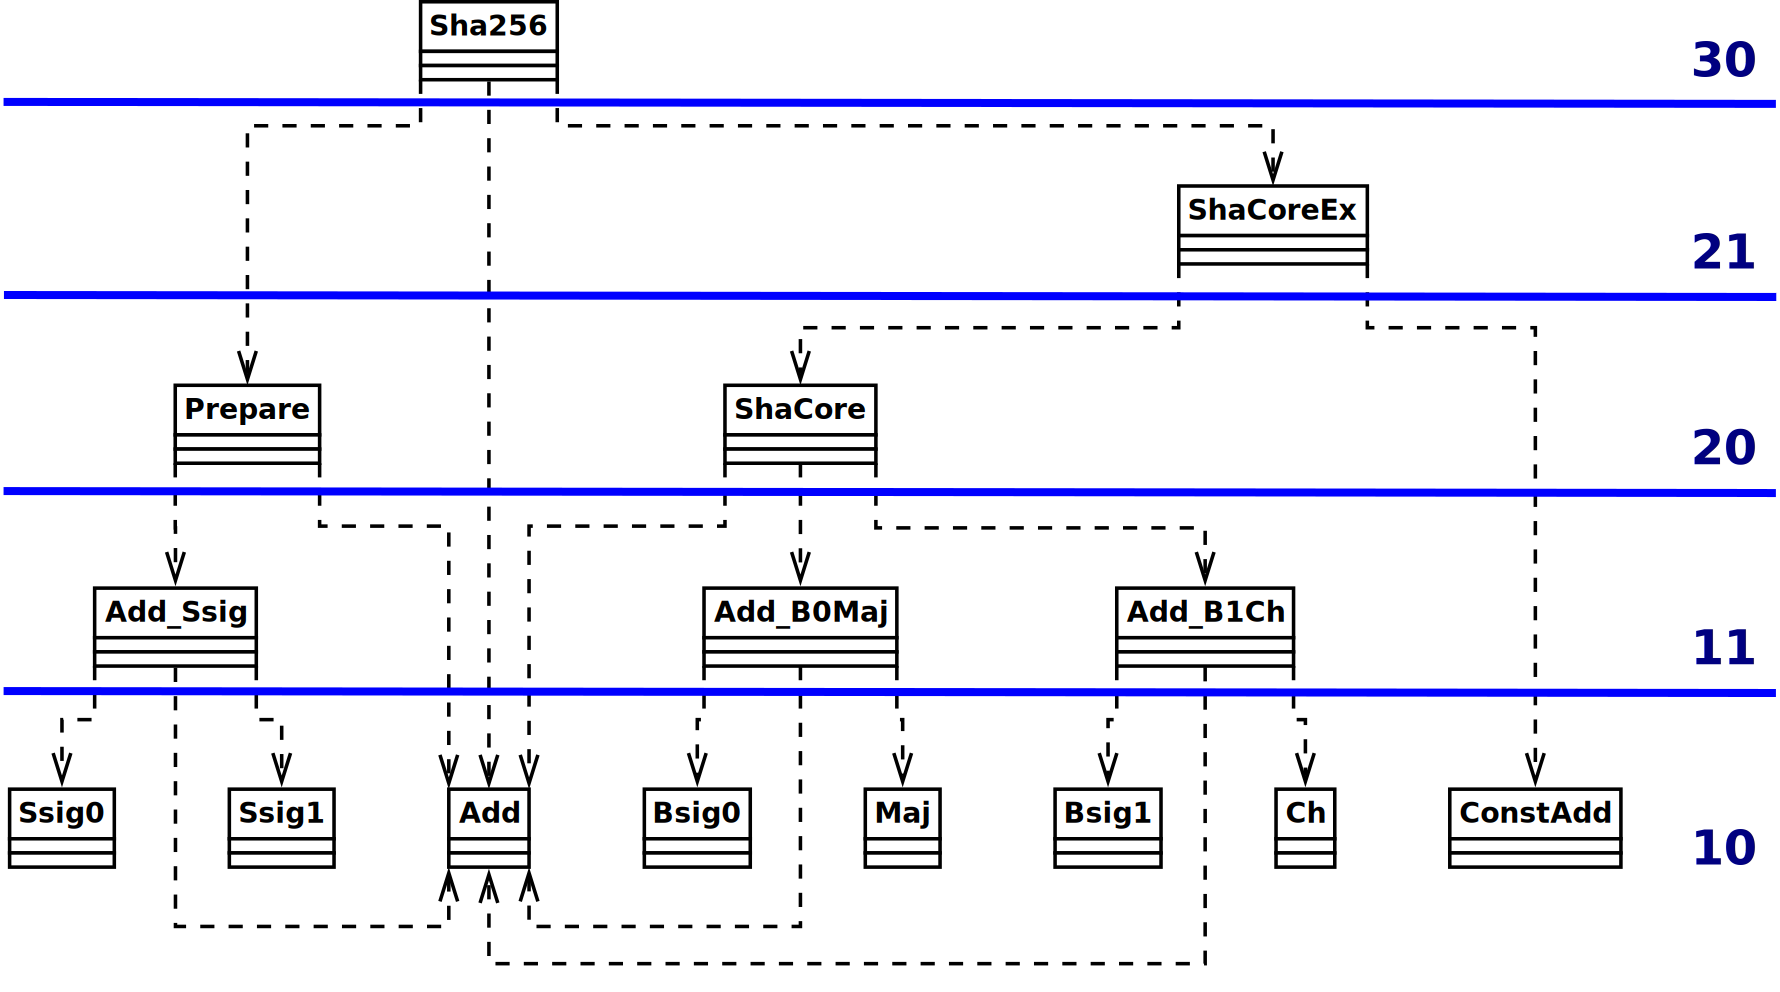
\includegraphics[scale=0.265]{images/module_level}
  \caption{Modullevel von \glos{sha256}}
  \label{fig:sha256_module_level}
\end{figure}

Die Level werden nicht fortlaufend nummeriert, um bei Bedarf weitere Module/Level einfügen zu können, ohne die Level der vorhandenen Module anpassen zu müssen.

Anhand der Level können die Module sortiert werden, so dass die Prüfung, ob eine Klausel zum Modul gehört, bei den Modulen mit dem niedrigsten Level beginnen kann.
Eine Klausel gehört dann zu einem Modul, wenn alle Literale der Klausel im Modul verwendet werden. Dabei kann es sich um Eingänge, zusätzliche Literale oder Ausgänge
handeln. Ein Sonderfall ist eine Klausel, die ausschließlich aus Eingangsliteralen oder ausschließlich aus Ausgangsliteralen besteht. Die Ausgangsliterale eines Moduls
sind im Allgemeinen die Eingangsliterale eines anderen Moduls, wodurch die Zuordnung bei gleichem Level unklar ist. Klauseln dieser Art wurden bei der Analyse jedoch
nicht gefunden. 

Für die Zuordnung der Klauseln wird zunächst ein Collector mit dem Namen "`ModulDB"' implementiert. Die ModulDB überschreibt nur die Methode newModul des Collectors,
um die Registrierung der Module zu erfassen. Generierte Klauseln, die an die Methode create übergeben werden, werden dadurch ignoriert. Erfasst werden neben dem
Modulnamen und dem Level die verwendeten Literale in der Reihenfolge: Eingänge, zusätzliche Literale und Ausgänge. ModulDB stellt außerdem eine Funktion bereit,
der eine beliebige Klausel zur Zuordnung übergeben werden kann. Wird ein passendes Modul gefunden, wird ein Zeiger auf die Modulinformationen zurückgeliefert.

Das Programm "`modulchecker"' nutzt schließlich die ModulDB für die Zuordnung. Zunächst wird ein Objekt der Kompressionsfunktion erzeugt, in das die ModulDB als
Besucher übergeben wird. Danach werden die im vorigen Abschnitt erstellten DIMACS-Dateien eingelesen und jede Klausel einem Modul zugeordnet. Die Zuordnung wird
in diesem Fall immer gelingen, weil spätestens die Kompressionsfunktion alle Literale umfasst.

Da die Module in ihrer Normalform implementiert werden (siehe Kapitel \ref{chp:knf}), kann eine zugeordnete Klausel noch nicht direkt genutzt werden.
Die verwendeten Literale in der Kompressionsfunktion sind andere als die des Moduls in der Normalform. Wird eine Klausel zugeordnet, erfolgt deshalb
direkt im Anschluss die Normalisierung der Klausel. Diese wird auf Basis der im Modul verwendeten Literale durchgeführt. Da diese in der richtigen
Reihenfolge vorliegen, können in der Klausel vorkommende Literale darin erkannt und anhand des Index in das Literal der Normalform überführt werden.

Nach der Normalisierung werden die Klauseln für jedes Modul in einem eigenen "`set"' gesammelt. Wie in Abschnitt \ref{sec:ana:rem_double} erfolgt
dadurch eine automatische Aussortierung doppelter Klauseln. Diese ist erneut notwendig, weil Module mehrfach an verschiedenen Stellen verwendet werden.
Klauseln, die vorher unterschiedlich sind, werden durch die Normalisierung zu gleichen Klauseln, wenn das gleiche Wissen über ein Modul an mehreren
Stellen erworben wurde.

Abschließend werden die neuen Klauseln jedes Moduls in eine eigene DIMACS-Datei geschrieben. Bevor diese Klauseln in die Module integriert werden können, ist
es notwendig die Gültigkeit zu überprüfen. Ungültig kann eine Klausel dann sein, wenn sie sich aus dem Kontext, in dem das Modul verwendet wurde, ergibt.
In diesem Fall ist es notwendig, die Klausel auf ein Modul höheren Levels zu übertragen. Die Gültigkeitsprüfung wird mit dem Programm "`clausechecker"'
durchgeführt. Dabei werden die bekannten Klauseln des Moduls an CryptoMiniSat übergeben. Jede (neue) Klausel lässt sich als nicht erfüllbare Belegung
interpretieren und wird deshalb als Annahme bei einem Lösungsversuch übergeben. Gelingt es CryptoMiniSat nicht, eine Lösung zu finden, ist die Gültigkeit
der Klausel bestätigt. In dieser Arbeit haben sich jedoch alle überprüften Klauseln als gültig herausgestellt und brauchen nicht auf ein Modul höheren
Levels übertragen zu werden.

Nur ein kleiner Teil (< 5\%) der neuen Klauseln lässt sich einem Modul unterhalb des Levels 30 zuordnen. Der Großteil ergibt sich aus dem Zusammenspiel
der Erweiterung der Eingabe und der Rundenfunktion und wird somit dem Modul für die Kompressionsfunktion zugeordnet. Der Versuch alle diese Klauseln
in einen weiteren Lösungsversuch einzubringen hat gezeigt, dass dadurch der Lösungsprozess deutlich verlangsamt wird. Daraus ergibt sich die Notwendigkeit,
diese Klauseln einer weiteren Analyse zu unterziehen, die im folgenden Abschnitt erläutert wird.
\section{Distanzermittlung von Klauseln außerhalb der Module}

\TODO{erledigen}
\section{Prüfung auf kürzere vorhandene Klauseln}

\TODO{erledigen}
\section{Auflistung gelernter Klauseln}
\label{sec:ana:overview}

\TODO{erledigen}